
\documentclass[11pt]{article}
\usepackage[a4paper,margin=1in]{geometry}
\usepackage{amsmath,amssymb}
\usepackage{graphicx}
\usepackage{booktabs,tabularx,longtable,array}
\usepackage{caption}
\usepackage{subcaption}
\usepackage{hyperref}
\usepackage{xcolor}
\usepackage{microtype}
\usepackage{enumitem}
\usepackage{float}
\hypersetup{colorlinks=true,linkcolor=blue,citecolor=blue,urlcolor=blue}
\newcommand{\mmals}{\textsc{MMALS}}
\newcommand{\rc}{\textsc{RC2O}}
\newcommand{\splitcifar}{\textsc{SplitCIFAR10}}
\title{\textbf{MMALS External Continual-Learning Bridge on SplitCIFAR10:\\Robust RC2O-v2.2c Evidence over Frozen Visual Feature Hosts}}
\author{Guillaume Harbonnier \\ MMALS Project}
\date{Robust addendum release: June 11, 2026}
\begin{document}
\maketitle
\begin{abstract}
This report updates the \mmals{} arXiv/GitHub companion package with the \rc{}-v2.2c robust \splitcifar{} addendum. The experiment is designed as an external continual-learning bridge: images are first mapped by a supervised A1 visual backbone into a frozen 256-dimensional feature representation, then the downstream \mmals{}/\rc{} continual-learning stack is evaluated on five disjoint class-incremental tasks. The robust run spans five seeds, eight epochs per task, and validation-selected baseline hardening against replay, EWC, LwF, PNN, and MoE-style controls. Selected \rc{} reaches $0.91395\pm0.00639$ final average accuracy, compared with $0.73860\pm0.01559$ for the best replay baseline. The paired gain against replay is $+0.17535$ with 95\% confidence interval $[0.16093,0.18977]$. The selected policy also reports min-task accuracy $0.8535$, average forgetting $0.02425$, min-class recall $0.8410$, and no zero-recall classes. The result supports a robust external continual-learning bridge over frozen supervised visual features. It does not claim end-to-end raw-pixel continual representation learning, CIFAR10 state of the art, or broad external-dataset generality.
\end{abstract}

\section{Purpose and claim boundary}
The purpose of this update is to freeze the \rc{}-v2.2c \splitcifar{} robust bridge result and integrate it into the paper and GitHub package accompanying the main \mmals{} and \rc{} articles. The claim boundary is deliberately narrow. The experiment tests the continual-learning, routing, memory, readout, and policy-selection layers of \mmals{} once a usable visual representation has been established. It does not test whether the visual backbone itself can be learned sequentially from raw pixels without forgetting.

\begin{table}[H]
\centering
\caption{Supported and unsupported claims.}
\begin{tabularx}{\linewidth}{lX}
\toprule
Status & Claim boundary \\
\midrule
Supported & Robust external SplitCIFAR10 CL bridge over frozen A1 visual features. \\
Supported & Selected RC2O beats validation-selected replay over five seeds. \\
Supported & Readout collapse is not observed for the selected policy: no zero-recall classes. \\
Supported as audit & Specialization diagnostics are materialized and aligned to the selected candidate. \\
Not claimed & End-to-end raw-pixel continual representation learning. \\
Not claimed & SOTA CIFAR10 performance or broad external-dataset generality. \\
Not claimed & Positive backward transfer as a demonstrated mechanism. \\
\bottomrule
\end{tabularx}
\end{table}

\section{Scientific demarche}
The experimental path began with weak raw-flat and early small-CNN SplitCIFAR runs. This created a serious confound: a poor continual-learning score could have come from a weak visual representation rather than from the \mmals{}/\rc{} mechanism. The robust package therefore follows a disciplined sequence: diagnose the representation bottleneck, harden the baselines, validate the A1 visual backbone, run the class-incremental CL protocol, and close the audit loop with selected-policy specialization diagnostics.

\begin{figure}[H]
\centering
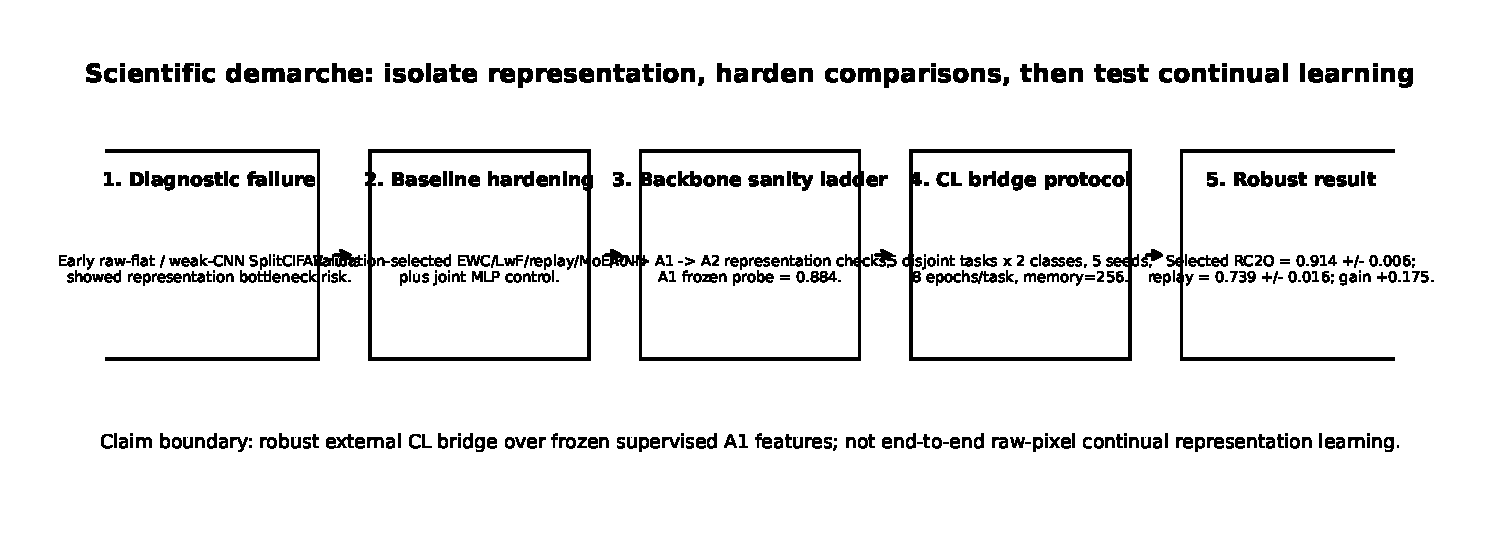
\includegraphics[width=0.98\linewidth]{figures/scientific_demarche_graph.pdf}
\caption{Scientific demarche used to move from representation debugging to robust external continual-learning evidence.}
\end{figure}

\section{Architecture: perceptual host and functional hosts}
The current experiment separates the perceptual host from the downstream functional \mmals{} hosts. Let $x$ denote a raw CIFAR10 image. A1 is a perceptual host
\begin{equation}
 e = \phi_A(x;\theta_A)\in\mathbb{R}^{256},
\end{equation}
trained and sanity-checked before the continual-learning sequence. During the CL experiment, $\theta_A$ is frozen. The downstream \mmals{} hosts then operate on $e$:
\begin{equation}
 z_k = H_k(e),\quad r_k = q_k(e,m,c),\quad z = \sum_k r_k z_k,\quad \hat{y}=h(z).
\end{equation}
The \rc{} controller is a policy selector over validation and audit-memory traces. It does not simply report the best final-test row; it selects a deployable family under regime and safety constraints.

\begin{figure}[H]
\centering
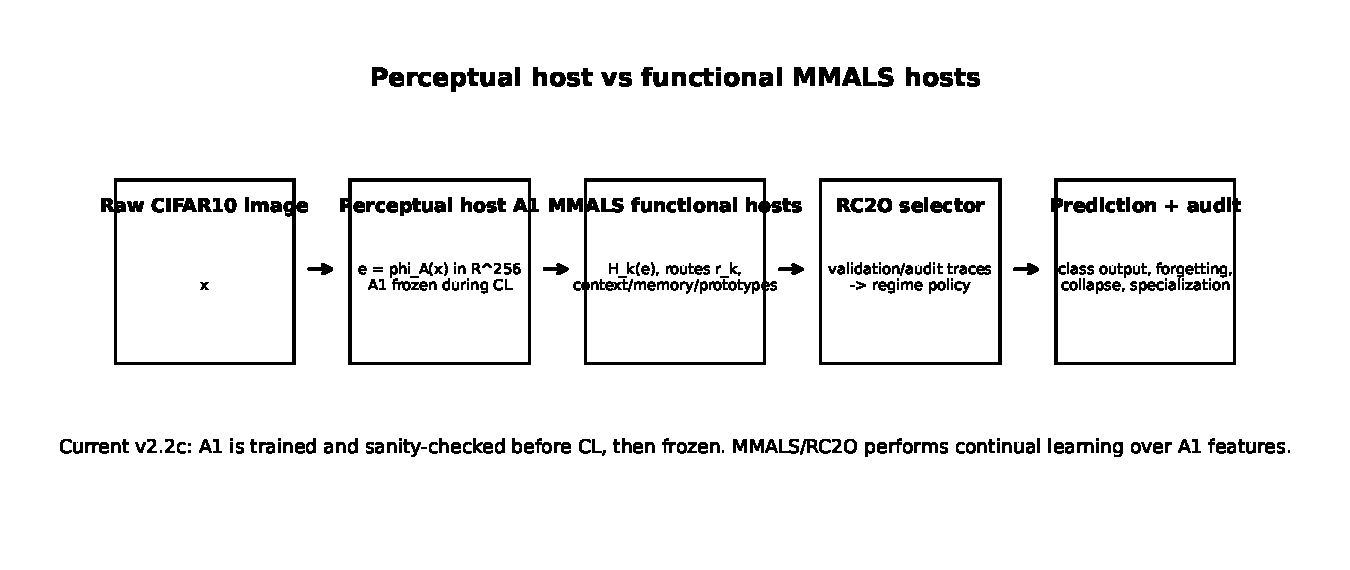
\includegraphics[width=0.95\linewidth]{figures/perceptual_host_pipeline.pdf}
\caption{Current v2.2c architecture: A1 is a frozen perceptual host; \mmals{} functional hosts, memory and policy selection perform continual learning over A1 features.}
\end{figure}

\section{Protocol}
The robust package uses five disjoint binary tasks over CIFAR10 classes:
\begin{equation}
(0,1)\rightarrow(2,3)\rightarrow(4,5)\rightarrow(6,7)\rightarrow(8,9).
\end{equation}
After each new task, all seen tasks are evaluated. Thus the evaluation chain is the standard continual-learning pattern: train on a new task, infer on old and new tasks, update memory and prototypes, then continue to the next task. The robust run uses seeds $\{0,1,2,3,4\}$, eight epochs per task, and memory size 256. Baseline hyperparameters are selected on validation memory, not by arbitrary defaults.

\section{Backbone sanity ladder}
The representation question is resolved by the A1 backbone sanity ladder. The A1 supervised backbone and A1 frozen linear probe both reach approximately $0.884$ in robust mode. This makes the downstream CL comparison meaningful: if \mmals{} failed after this point, the most plausible source would be memory, readout, routing or selector behavior, not a visibly broken visual feature extractor.

\begin{figure}[H]
\centering
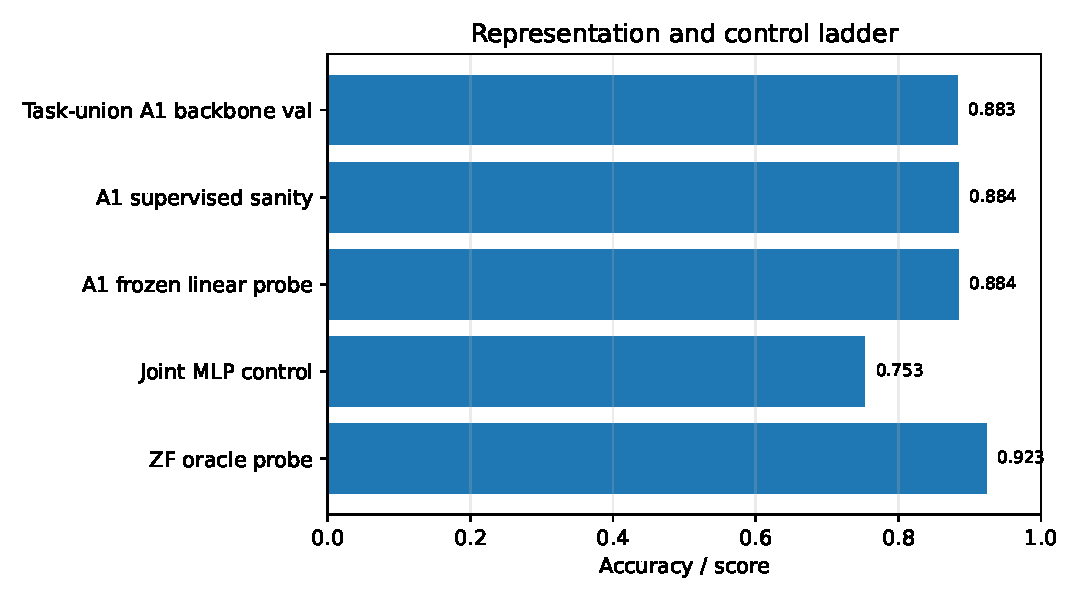
\includegraphics[width=0.75\linewidth]{figures/representation_ladder_paper.pdf}
\caption{Representation and control ladder in the robust package. The row named joint upper bound in the raw notebook is interpreted here as a joint MLP control, not as a theoretical upper bound.}
\end{figure}

\begin{table}[H]
\centering
\caption{Representation ladder and controls.}
\begin{tabularx}{\linewidth}{lcccc}
\toprule
Stage & Metric & Value & Secondary & Diagnostic \\
\midrule
Task-union A1 backbone val & feature\_backbone\_val\_acc & 0.8831 & 0.8987 & yes \\
A1 supervised sanity & val\_acc\_best & 0.8844 & 0.8797 & yes \\
A1 frozen linear probe & val\_acc\_best & 0.8841 & 0.8803 & yes \\
Joint MLP control & final\_avg\_acc\_mean & 0.7531 & -- & no \\
ZF oracle probe & probe\_proto\_\_zf\_oracle & 0.9234 & -- & yes \\
\bottomrule
\end{tabularx}
\end{table}

\section{Robust results}
Table~\ref{tab:leaderboard} reports the robust 5-seed leaderboard. Selected \rc{} is close to the ZF oracle probe and clearly above the best replay baseline. The safe readout candidate is essentially tied with the selected policy, which is useful because it indicates that the selected policy is not a brittle outlier.

\begin{figure}[H]
\centering
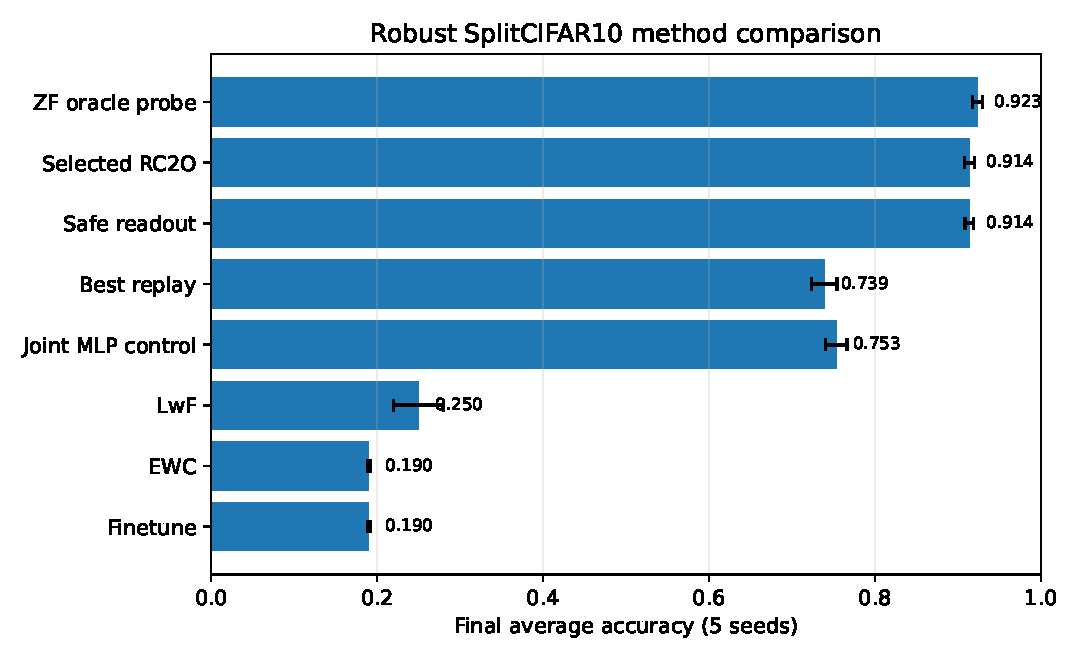
\includegraphics[width=0.80\linewidth]{figures/robust_method_comparison.pdf}
\caption{Robust method comparison over five seeds. Error bars denote standard deviation where available.}
\end{figure}

\begin{table}[H]
\centering
\caption{Robust method leaderboard.}
\label{tab:leaderboard}
\begin{tabularx}{\linewidth}{lccccc}
\toprule
Method & Final avg. acc. & Min-task & Forgetting & Min-class & Size MB \\
\midrule
Selected RC2O & 0.9140 $\pm$ 0.0064 & 0.8535 & 0.0242 & 0.8410 & 2.011 \\
Safe readout & 0.9139 $\pm$ 0.0054 & 0.8530 & 0.0239 & 0.8430 & 2.011 \\
RC1b guarded context gap & 0.9097 $\pm$ 0.0081 & 0.8470 & 0.0298 & 0.8285 & 2.011 \\
ZF oracle probe & 0.9234 $\pm$ 0.0059 & 0.8678 & -- & 0.8270 & 0.002 \\
ZF proto probe & 0.9206 $\pm$ 0.0086 & 0.8642 & -- & 0.8140 & 0.002 \\
Best replay & 0.7386 $\pm$ 0.0156 & 0.6020 & 0.1921 & 0.5665 & 0.316 \\
Joint MLP control & 0.7531 $\pm$ 0.0132 & 0.6245 & 0.0000 & 0.5795 & 0.316 \\
Finetune & 0.1897 $\pm$ 0.0017 & 0.0000 & 0.9306 & 0.0000 & 0.316 \\
EWC & 0.1899 $\pm$ 0.0016 & 0.0000 & 0.9346 & 0.0000 & 0.316 \\
LwF & 0.2498 $\pm$ 0.0299 & 0.0380 & 0.0039 & 0.0005 & 0.316 \\
\bottomrule
\end{tabularx}
\end{table}

\subsection{Per-seed stability}
The paired selected-RC2O gain over replay is positive in every seed. The average gain is $+0.17535$ with 95\% confidence interval $[0.16093,0.18977]$. The oracle gap remains small, averaging $0.0095$.

\begin{figure}[H]
\centering
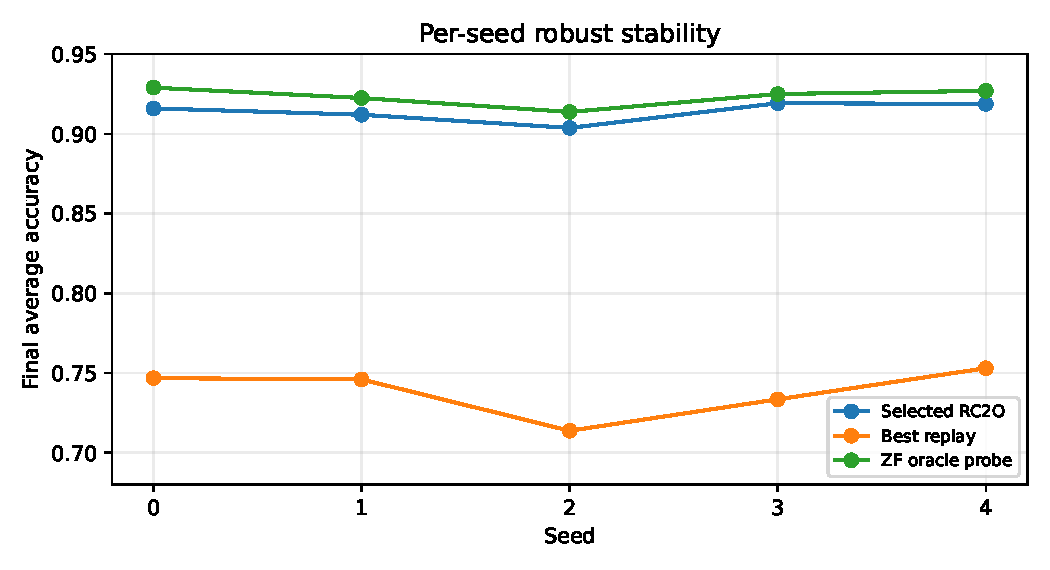
\includegraphics[width=0.80\linewidth]{figures/per_seed_robust_accuracy.pdf}
\caption{Per-seed accuracy of selected RC2O, best replay and the oracle probe.}
\end{figure}

\begin{table}[H]
\centering
\caption{Per-seed robust comparison.}
\begin{tabularx}{\linewidth}{cccccccc}
\toprule
Seed & Selected & Safe & Replay & Joint ctrl. & Oracle & $\Delta$ vs replay & Oracle gap \\
\midrule
0 & 0.9160 & 0.9130 & 0.7468 & 0.7605 & 0.9290 & 0.1693 & 0.0130 \\
1 & 0.9120 & 0.9120 & 0.7460 & 0.7465 & 0.9225 & 0.1660 & 0.0105 \\
2 & 0.9038 & 0.9062 & 0.7137 & 0.7627 & 0.9137 & 0.1900 & 0.0100 \\
3 & 0.9193 & 0.9193 & 0.7335 & 0.7330 & 0.9250 & 0.1857 & 0.0057 \\
4 & 0.9187 & 0.9187 & 0.7530 & 0.7630 & 0.9270 & 0.1657 & 0.0083 \\
\bottomrule
\end{tabularx}
\end{table}

\section{Baseline hardening}
A central reviewer risk in earlier runs was that replay, EWC, LwF, PNN or MoE controls could be dismissed as arbitrary defaults. The v2.2c robust package addresses this by exporting a validation-memory baseline hardening trace. For each seed, baseline candidates are selected by validation score before the final comparison. This makes the baseline comparison stronger, though it is still not a claim of state-of-the-art baseline tuning.

\begin{table}[H]
\centering
\caption{Validation-selected baseline hardening summary.}
\begin{tabularx}{\linewidth}{lccccc}
\toprule
Baseline family & Selected seeds & Val. score & Val. final avg & Val. min-task & Val. forgetting \\
\midrule
balanced\_replay & 5 & 0.7238 & 0.6973 & 0.5577 & 0.1171 \\
experience\_replay & 5 & 0.7238 & 0.6973 & 0.5577 & 0.1171 \\
lwf & 5 & 0.2289 & 0.2285 & 0.0190 & 0.0063 \\
sparse\_moe & 5 & 0.0066 & 0.1759 & 0.0000 & 0.6769 \\
pnn & 5 & 0.0062 & 0.1746 & 0.0000 & 0.6737 \\
noisy\_topk\_moe & 5 & 0.0059 & 0.1751 & 0.0000 & 0.6765 \\
ewc & 5 & 0.0051 & 0.1753 & 0.0000 & 0.6806 \\
hard\_top1\_moe & 5 & 0.0050 & 0.1729 & 0.0000 & 0.6715 \\
dense\_moe & 5 & 0.0043 & 0.1737 & 0.0000 & 0.6777 \\
finetune & 5 & 0.0040 & 0.1733 & 0.0000 & 0.6771 \\
joint\_upper\_bound & 5 & -- & -- & -- & -- \\
\bottomrule
\end{tabularx}
\end{table}

\section{Readout collapse, min-class behavior and forgetting}
The selected policy reports min-task accuracy $0.8535$, average forgetting $0.02425$, min-class recall $0.8410$, and no zero-recall classes. These values matter because early SplitCIFAR runs were often dominated by class collapse or task collapse. The robust result is therefore not merely a high average-accuracy row; it is also a non-collapse result.

\section{Selected-policy specialization audit}
The v2.2c patch fixed a previous audit gap: route/context, host ablation, host probe and prototype separation are now aligned to the selected policy candidate when available. The robust run materializes all four components across seeds.

\begin{table}[H]
\centering
\caption{Specialization audit materialization and selected-policy alignment.}
\begin{tabularx}{\linewidth}{lcccc}
\toprule
Component & OK seeds & Rows & Total rows & Aligned \\
\midrule
host\_ablation & 5 & 5 & 150 & yes \\
host\_probe & 5 & 5 & 125 & yes \\
prototype\_separation & 5 & 5 & 50 & yes \\
route\_context\_and\_confusion & 5 & 5 & 50 & yes \\
\bottomrule
\end{tabularx}
\end{table}

\section{SplitCIFAR10 external-bridge gate}
The raw notebook exports a SplitCIFAR10-specific external-bridge gate. This gate is not a MNIST-family robust gate; it checks whether the bridge experiment is interpretable: A1 passes representation sanity, the joint MLP control is no longer collapsed, selected RC2O is competitive with hardened replay, min-task and min-class metrics are non-collapsed, and specialization components are present.

\begin{table}[H]
\centering
\caption{SplitCIFAR10 external-bridge gate.}
\begin{longtable}{p{0.47\linewidth}cccc}
\toprule
Check & Value & Floor & Ceiling & Status \\
\midrule
\endfirsthead
\toprule
Check & Value & Floor & Ceiling & Status \\
\midrule
\endhead
a1\_supervised\_backbone\_pass & 0.8844 & 0.6500 & -- & PASS \\
a1\_frozen\_linear\_probe\_pass & 0.8841 & 0.5500 & -- & PASS \\
joint\_upper\_bound\_representation\_floor & 0.7531 & 0.5500 & -- & PASS \\
selected\_rc2o\_competitive\_with\_replay & 0.9140 & 0.7286 & -- & PASS \\
selected\_min\_task\_nonzero & 0.8535 & 0.0500 & -- & PASS \\
selected\_forgetting\_not\_explosive & 0.0242 & -- & 0.2000 & PASS \\
selected\_min\_class\_nonzero & 0.8410 & 0.0500 & -- & PASS \\
selected\_zero\_recall\_classes\_gate & -- & -- & 0.0000 & PASS \\
specialization\_components\_materialized & 4.0000 & 4.0000 & -- & PASS \\
specialization\_aligned\_to\_selected\_policy & 1.0000 & 1.0000 & -- & PASS \\
\bottomrule
\end{longtable}
\end{table}

\section{Discussion}
This result upgrades \splitcifar{} from a representation-debugging branch to a robust external CL bridge. The strongest scientific contribution is not that \mmals{} is now a universal continual-learning solution. The contribution is narrower and stronger: once the representation bottleneck is controlled and baselines are validation-hardened, the \mmals{}/\rc{} stack robustly preserves high accuracy and low forgetting over the SplitCIFAR10 sequence.

Two caveats are central. First, the visual backbone is frozen during continual learning. This isolates the downstream memory and routing layers, but it does not validate end-to-end raw-pixel continual representation learning. Second, the row originally named joint upper bound should be renamed joint MLP control. Because selected \rc{} exceeds it, it cannot be interpreted as a mathematical upper bound. It is a useful control with the same readout scale, not a ceiling.

\section{Limitations and next steps}
The immediate next step is not to expand the claim, but to repeat the same discipline on harder data. The recommended sequence is: freeze this \splitcifar{} robust bridge; update the main \mmals{} and \rc{} companion papers; then move to SplitCIFAR100, CORe50, TinyImageNet or DomainNetMini with the same baseline-hardening and representation-ladder discipline. A stronger future version would promote the A1 perceptual host into a slow-plasticity host, constrained by feature-stability, prototype-stability and context-consistency losses.

\section{Reproducibility package}
The GitHub package contains the LaTeX source, compiled PDF, figures, tables, robust CSV/JSON summaries, selected raw CSV artifacts, the v2.2c notebook, and the robust analysis report. The included README documents the build command and claim boundary.

\bibliographystyle{plain}
\bibliography{references}
\end{document}
